% !TeX root = ..\dokumentation.tex

\chapter{Technische Umsetzung}
In diesem Kapitel wird die technische Umsetzung der Plattform Skiosa betrachtet.
\todo{to be changed}

\section{Infrastruktur}
\todo{}

\subsection{Datenpersistenz}
Um persistente Daten auf der Plattform zu haben, wurde PostgreSQL \parencite{web/postgresql} als Datenbank verwendet.
Die Datendefinition wurde durch TypeORM \parencite{web/TypeORM} dargestellt.
Es wurden die Article von RSS-Feeds in dem Schema aus Abbildung~\ref{fig:databaseORM} abgebildet.
\begin{figure}
    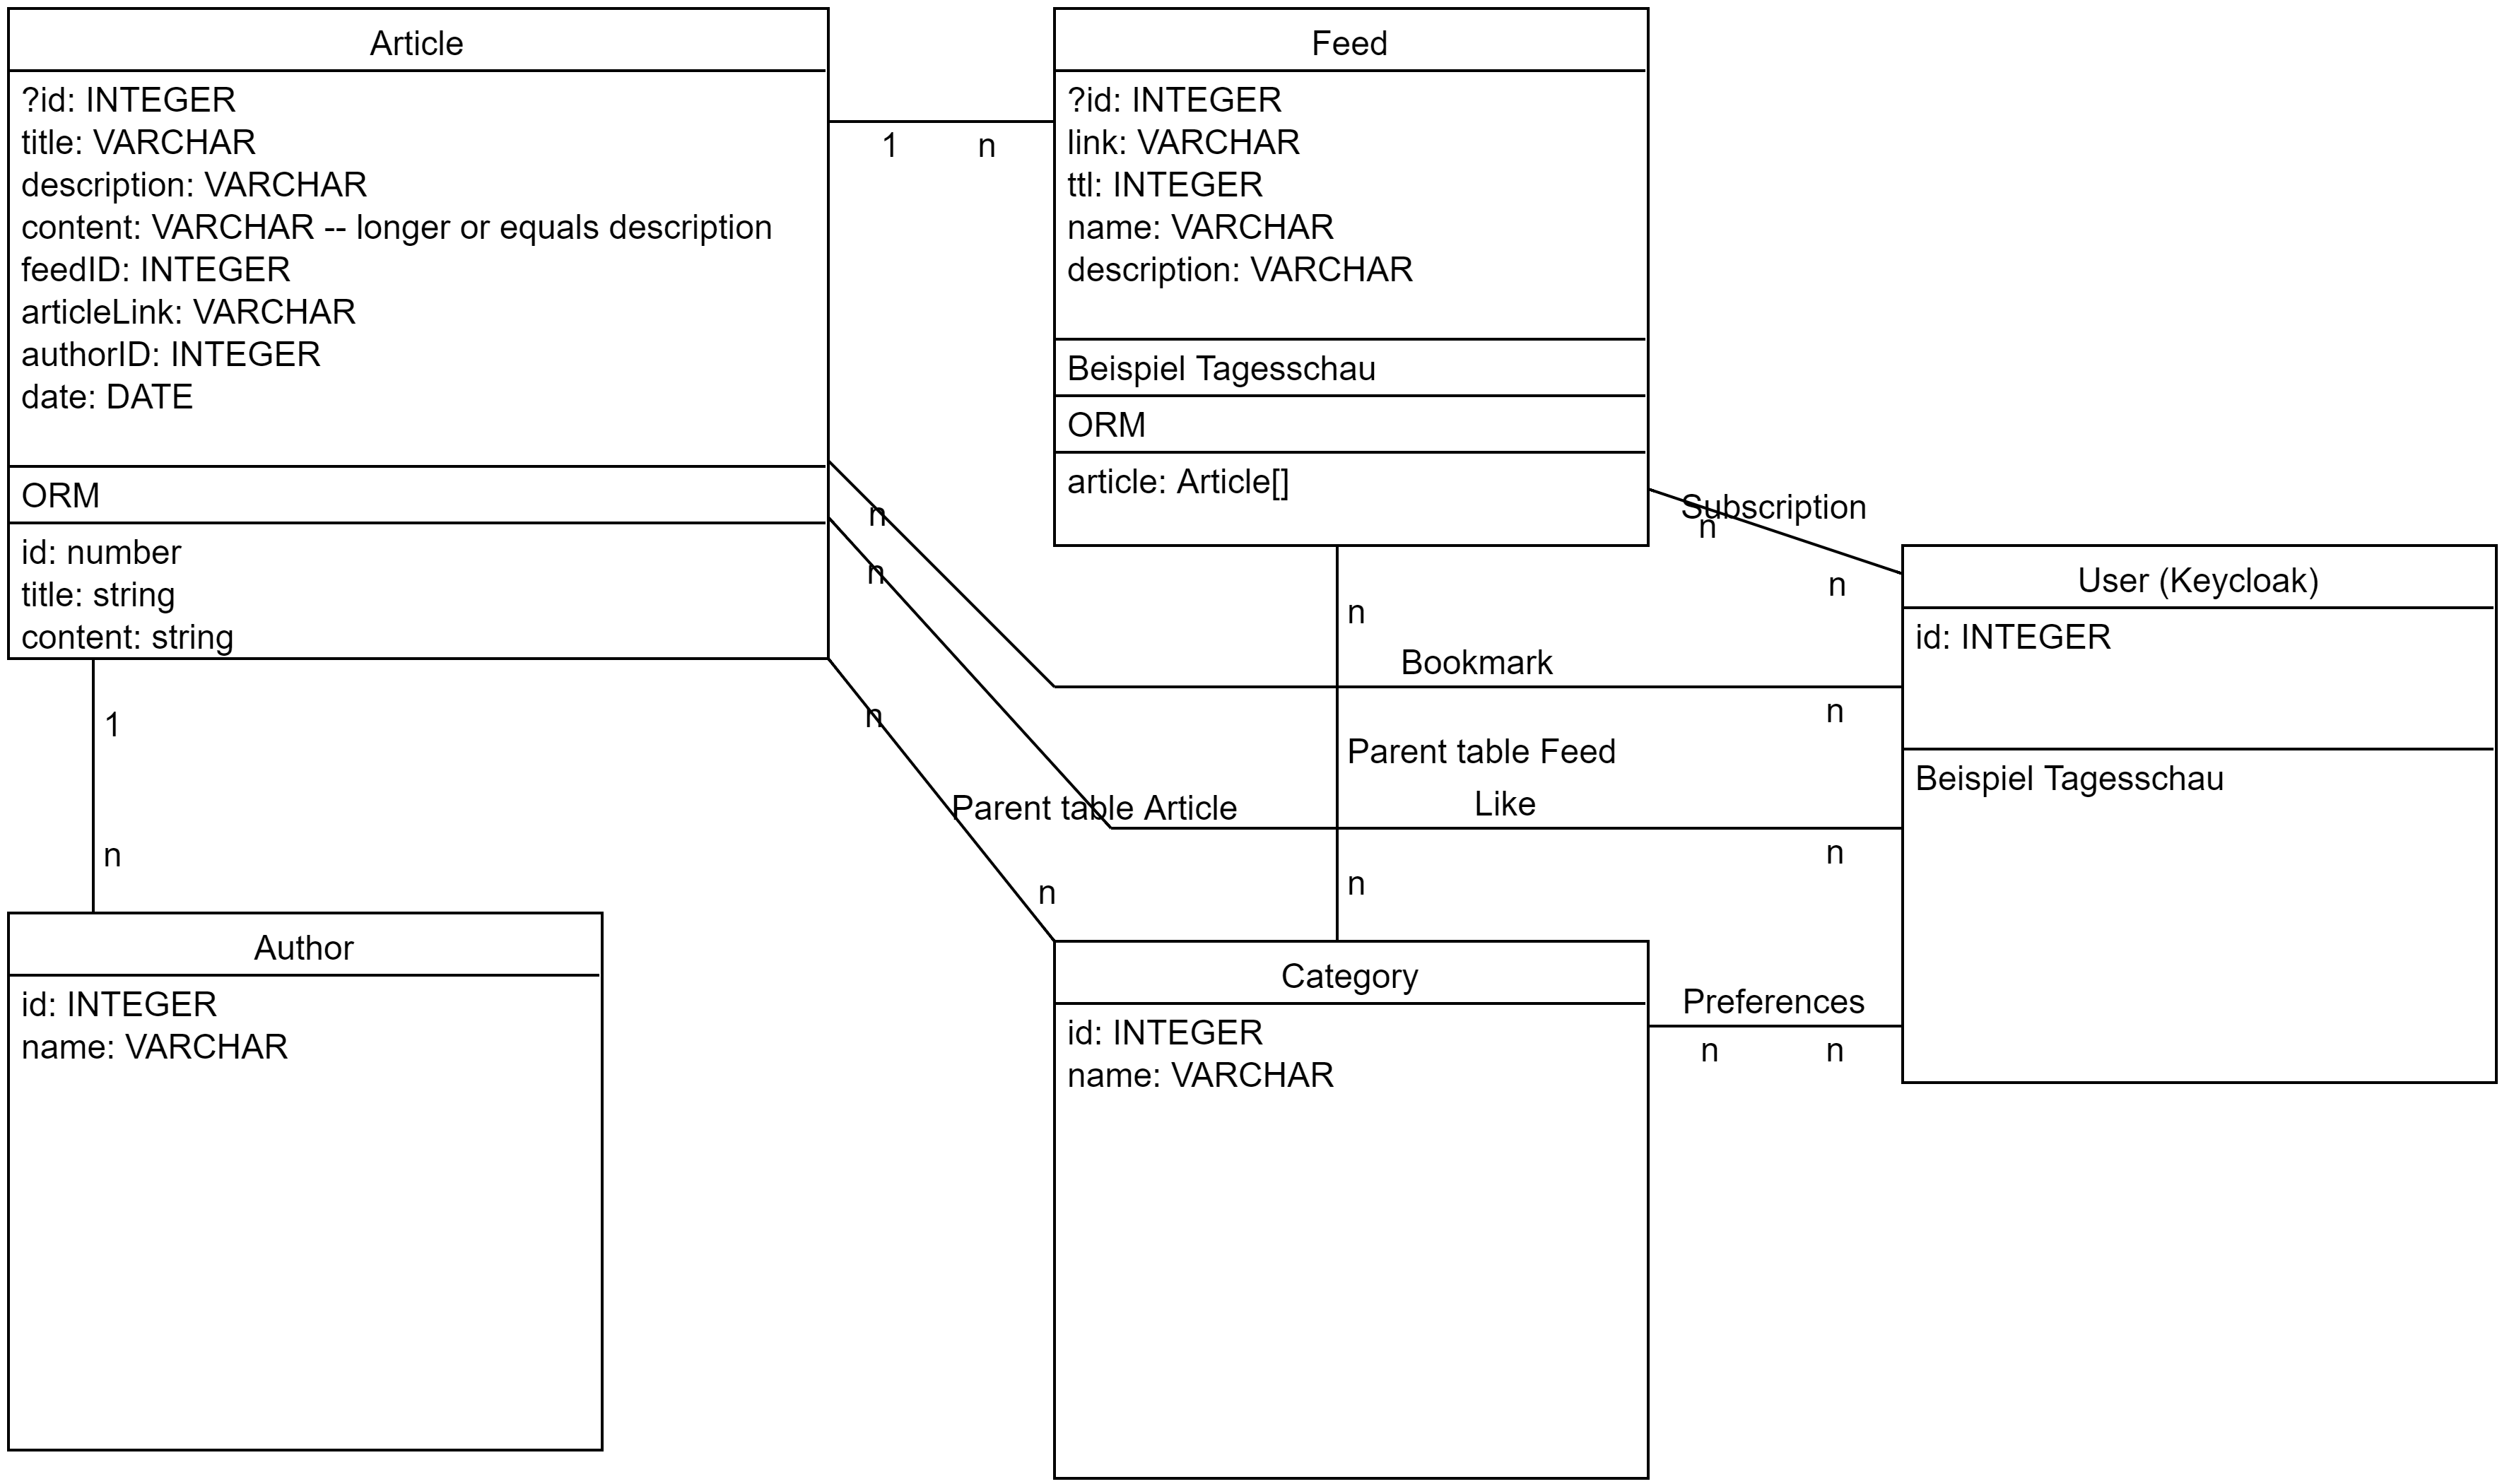
\includegraphics[width=\linewidth]{Database_Model.png}
    \caption{Datendefinition innerhalb der Datenbank}
    \label{fig:databaseORM}
\end{figure}